\documentclass[manuscript]{article}

\usepackage{graphicx}
\usepackage{epsfig}
\usepackage{amssymb}
\usepackage{amsmath}
\newcommand\numberthis{\addtocounter{equation}{1}\tag{\theequation}}
\usepackage{psfrag}
\usepackage{color}
\usepackage{epstopdf}
\usepackage{hyperref}

%%%
\begin{document}

\title{SVM algorithm to predict Titanic survivors.}

\author{Alexandre Caz\'e}
\maketitle

\begin{abstract}
Given data on 891 passengers of the Titanic (age, class, sex, ...), the Kaggle tutorial "Titanic: Machine Learning from Disaster" (\url{http://www.kaggle.com}) asks to predict the survival of 418 other passengers. 
In this note, we present our results using the Support Vector Machine (SVM) algorithm LinearSVC provided by the library sklearn in python. 
After a raw overview on the data, we only take into account two features, that are Gender and Class.
We show that this algorithm leads to a model where all women survive and all men die, independently on the class.
This leads to a prediction efficiency of 0.76555 in the Kaggle leaderboard, which corresponds to the benchmark "Gender based model".
\end{abstract}

%%%

% 1 - Overlook on the data and first conclusions
\section{Overlook on the data and first conclusions}

	% 1.1 - Features
	\subsection{Features}
	
We restrict ourself to three features of the data: Gender, Class and Adult. 
%
\begin{itemize}
\item Gender: Male or Female.
\item Class: 1st, 2nd or 3rd class.
\item Adult: Adult (over 18) or Child (under 18).
\end{itemize}

	% 1.2 - Statistics
	\subsection{Statistics}

Some first statistics describing the data are presented in the following tables:
%
\begin{itemize}
\item Table~\ref{tab:comparison} sums up the general statistics of the training and test sets.
\item Table~\ref{tab:survival_rates} sums up the survival rates depending on each feature individually.
\item Table~\ref{tab:Gender_Adult} describes the interaction between the features Gender and Adult for the survival rate.
\item Table~\ref{tab:Gender_Class} describes the interaction between the features Gender and Class for the survival rate.
\item Table~\ref{tab:Adult_Class} describes the interaction between the features Adult and Class for the survival rate.
\end{itemize}

\newpage

%
% Table 1: General stats
\begin{table}[h!]
\centering
\begin{tabular}{|c|c|c|}
\hline
& Training set & Test set \\
\hline
\# passengers & 891 & 418 \\
\hline
Adults & 84.4 \% & 87.1 \% \\
Children & 15.6 \% & 12.9 \%\\
\hline
Male & 64.8 \% & 63.6 \% \\
Female & 35.2 \% & 36.4 \% \\
\hline
1st class & 24.2 \% & 25.6 \% \\
2nd class & 20.7 \% & 22.2 \% \\
3rd class & 55.1 \% & 52.2 \% \\
\hline
\end{tabular}
\caption{Comparison Training set / Test set.}
\label{tab:comparison}
\end{table}
%
% Table 2: Survival rates
\begin{table}[h!]
\centering
\begin{tabular}{|c|c|}
\hline
Total & 0.384 \% \\
\hline
Adults & 0.362 \% \\
Children & 0.504 \%�\\
\hline
Male & 0.189 \% \\
Female & 0.742 \% \\
\hline
1st class & 0.63 \%�\\
2nd class & 0.473 \%�\\
3rd class & 0.242 \%�\\
\hline
\end{tabular}
\caption{Survival rates for each feature individually.}
\label{tab:survival_rates}
\end{table}
%
% Table 3: Interaction Gender / Adult
\begin{table}[h!]
\centering
\begin{tabular}{|c|c|c|c|}
\hline
& Male & Female & Total \\
\hline
Adults & 16.8 \% & 76.0 \% & 36.2 \% \\
Children & 33.8 \%�& 67.6 \% & 50.4 \% \\
\hline
Total & 18.9 \% & 74.2 \% & 38.4 \% \\
\hline
\end{tabular}
\caption{Survival rates : Interaction Gender / Adult.}
\label{tab:Gender_Adult}
\end{table}
%
% Table 4: Interaction Gender / Class
\begin{table}[h!]
\centering
\begin{tabular}{|c|c|c|c|}
\hline
& Male & Female & Total \\
\hline
1st class & 36.9 \% & 96.8 \% & 63.0 \% \\
2nd class & 15.7 \%�& 92.1 \% & 47.3 \% \\
3rd class & 13.5 \%�& 50.0 \% & 24.2 \% \\
\hline
Total & 18.9 \% & 74.2 \% & 38.4 \% \\
\hline
\end{tabular}
\caption{Survival rates : Interaction Gender / Class.}
\label{tab:Gender_Class}
\end{table}
%
% Table 5: Interaction Adult / Class
\begin{table}[h!]
\centering
\begin{tabular}{|c|c|c|c|}
\hline
& Adult & Child & Total \\
\hline
1st class & 61.0 \% & 87.5 \% & 63.0 \% \\
2nd class & 41.3 \%�& 79.3 \% & 47.3 \% \\
3rd class & 21.7 \%�& 35.1 \% & 24.2 \% \\
\hline
Total & 36.2 \% & 50.4 \% & 38.4 \% \\
\hline
\end{tabular}
\caption{Survival rates : Interaction Adult / Class.}
\label{tab:Adult_Class}
\end{table}

\newpage

	% 1.3 - First conclusions
	\subsection{First conclusions}
	 
From those statistics, one can draw some first raw conclusions:
%
\begin{itemize}
\item From Table~\ref{tab:survival_rates}, one can predict that the importance of the features will be in descending order Gender, then Class and finally Adult. The moto "Ladies and Children first" seems to have worked extremely well for female passengers, not so well for children. 
\item The low number of children that appears in Table~\ref{tab:comparison} may weaken any conclusion for the feature Adult.
\item From Table~\ref{tab:Gender_Class}, one can see that being a woman in first or second class was nearly the insurance to survive, while being a man was bad news in any class (although 1st class were not that desperate).
\end{itemize}

Given those first conclusions, we focus on the model that should be the most relevant, that is the Gender/Class model.

% 2 - SVM for the Gender/Class model
\section{SVM for the Gender/Class model}
	
Figure~\ref{fig:Gender_Class} shows the result of the LinearSVC algorithm from the library svm of sklearn (\url{http://scikit-learn.org/stable/modules/svm.html}).
The Python code that generates this figure is available on Github at \url{https://github.com/alexandrecaze/kaggle-titanic} (file svm.py).
%
\begin{figure}[h!]
\begin{center}
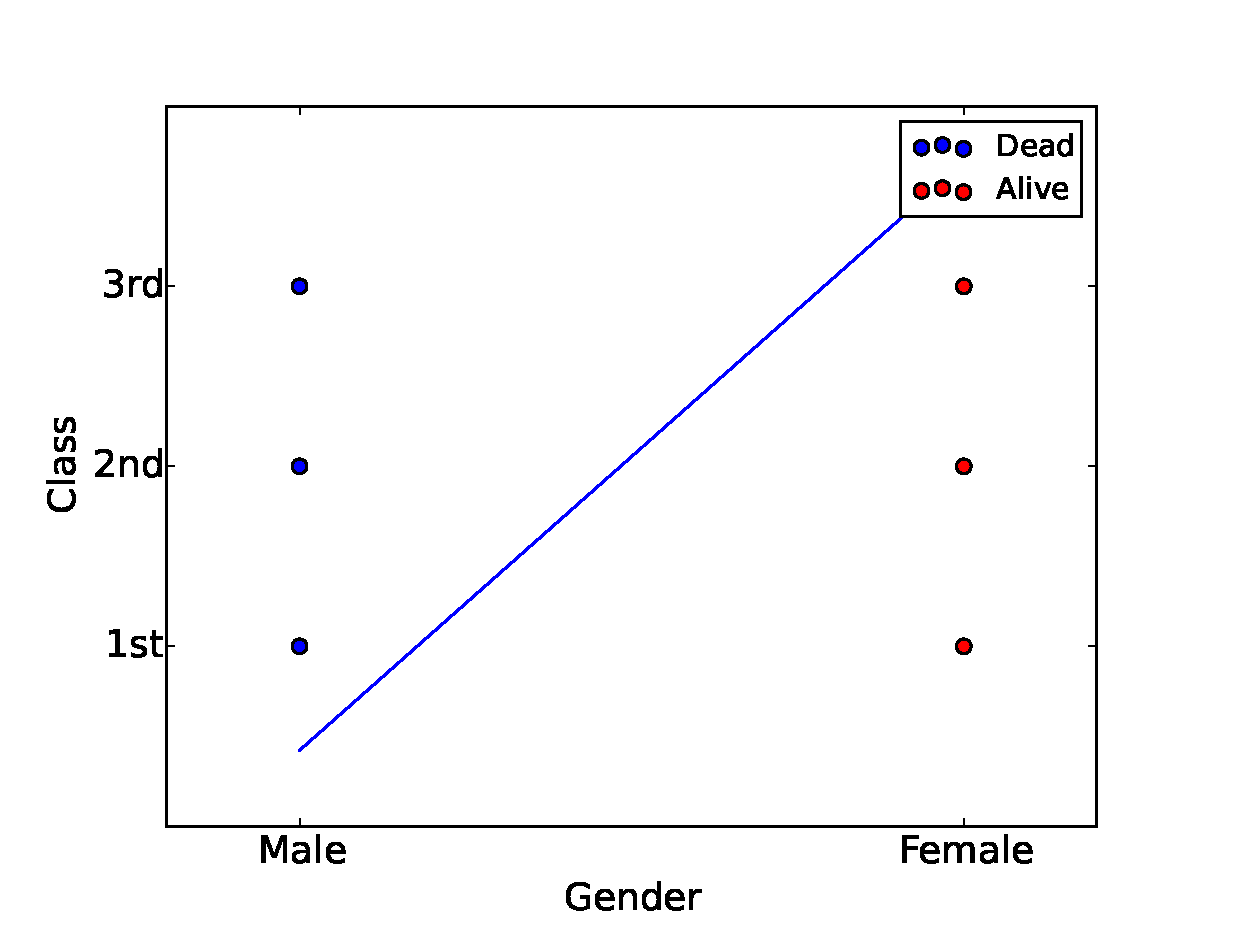
\includegraphics[width=\textwidth]{./GenderClass.eps}
\caption{\label{fig:Gender_Class} Separating line between survivors and non-survivors according to the SVM model based on the Gender/Class model.}
\end{center}
\end{figure}

In Fig.~\ref{fig:Gender_Class}, we have represented the 6 possible cases corresponding to the Gender-Class model (Male and 1st class, Male and 2nd class, ...) and the associated prediction according to the LinearSVC algorithm trained on the training set described in Table~\ref{tab:comparison}. 
Survivors are represented in red and non-survivors in blue. 
Note that this problem is not linearly separable, which implies non-trivial calculations in the black-box LinearSVC (for details, see e.g. Ref.~\cite{HastieBook}) in order to find the line that minimises the error, represented in blue.
As a conclusion, one can see that the best model in that framework ignores the feature Class and only predicts that women survive and men die.
This leads to a prediction efficiency of 76.555\% in the Kaggle leaderboard, calculated on the test set.
Although it might sound like a trivial result, it is elegant to obtain a mathematical justification for it (it is a close call for the women of 3rd class to be predicted as survivors, another training set using the same algorithm could have led to a different model).

%% Bibliography
% ============
\begin{thebibliography}{40}

\bibitem{HastieBook}
T. Hastie, R. Tibshirani and J. Friedman, {\it The Elements of Statistical Learning: Data Mining, Inference, and Prediction, Second Edition} (Springer Series in Statistics).

\end{thebibliography}

\end{document}
